\documentclass{../../templates/lkx_pset}

\title{Astron 140 Problem Set 7}
\author{Lev Kruglyak}
\due{November 5, 2024}

\usepackage{mdframed}


\usepackage[T1]{fontenc}
\RequirePackage{mlmodern}


\mdfdefinestyle{answer}{%
	linecolor=black,
	outerlinewidth=2pt,
	%roundcorner=20pt,
	innertopmargin=4pt,
	innerbottommargin=4pt,
	innerrightmargin=4pt,
	innerleftmargin=4pt,
	leftmargin = 4pt,
	rightmargin = 4pt
	%backgroundcolor=gray!50!white}
}

\newenvironment{answerbox}{
	\begin{mdframed}[style=answer,nobreak=true,userdefinedwidth=30em]}{\end{mdframed}}

\usepackage{siunitx}
\providecommand{\unitsi}[1]{\qty[per-mode = symbol]{#1}{}}
\providecommand{\mpssi}[1]{\qty[per-mode = symbol]{#1}{\m\per\s}}
\providecommand{\mpsssi}[1]{\qty[per-mode = symbol]{#1}{\m\per\s^2}}
\providecommand{\Gsi}[1]{\qty[per-mode = symbol]{#1}{\m^3\per\s^2\kg}}
\providecommand{\kBsi}[1]{\qty[per-mode = symbol]{#1}{\m^2\s^{-2}\K^{-1}\kg}}
\providecommand{\hsi}[1]{\qty[per-mode = symbol]{#1}{\J\cdot s}}
\providecommand{\kgsi}[1]{\qty[per-mode = symbol]{#1}{\kg}}
\providecommand{\ssi}[1]{\qty[per-mode = symbol]{#1}{\s}}
\providecommand{\psssi}[1]{\qty[per-mode = symbol]{#1}{\s^{-2}}}
\providecommand{\msi}[1]{\qty[per-mode = symbol]{#1}{\m}}
\providecommand{\desi}[1]{\qty[per-mode = symbol]{#1}{\J\per \m^3}}

\renewcommand{\O}{\mathrm{O}}
\providecommand{\Aff}{\mathrm{Aff}}
\providecommand{\SO}{\mathrm{SO}}

\providecommand{\Frame}{\mathrm{Fr}}

\providecommand{\A}{\mathbb{A}}

\providecommand{\definefunction}[5]{
	\begin{array}{rcl}
		#1 : #2 & \xrightarrow{\phantom{---}} & #3 \\
		#4      & \xmapsto{\phantom{---}}     & #5
	\end{array}
}


\providecommand{\pp}[2]{\frac{\partial #1}{\partial #2}}


\begin{document}
\maketitle

\begin{problem}{1}
In the analyses of the Mercury perihelion precession, we compared two cases, namely the case with or without the GR correction term, respectively. Schematically review the final solutions $\delta r(\phi)$ for these two cases (no derivation is necessary), and point out what is the key difference between the two solutions that leads to the precession.
\end{problem}

\begin{solution}
	In the Newtonian case, the pertubation in the orbital radius $\delta u(\phi)$ where $u=1/r$ takes the form
	\[
		\delta u(\phi) = \sqrt{A_{\textrm{newt}}} \sin(\phi + \phi_0)\quad\textrm{where}\quad A_{\textrm{newt}} = \frac{\widetilde{E}^2}{\widetilde{L}^2} - \frac{G^2M^2}{\widetilde{L}^4} - \frac{1}{\widetilde{L}^2}.
	\]
	When we include the GR correction term in the initial setup of the differential equations, we get
	\[
		\begin{aligned}
			\delta u(\phi) = \sqrt{A_{\textrm{GR}}} \sin(\sqrt{k}\phi + \phi_0) + a\quad\textrm{where}\quad A_{\textrm{GR}} &= A_{\textrm{newt}}^2 + \frac{2G^4M^4}{\widetilde{L}^6} + k\frac{9G^6M^6}{\widetilde{L}^2}\\
			k &= 1-\frac{6G^2M^2}{\widetilde{L}^2},\quad a = \frac{3G^3M^3}{\widetilde{L}^4}.
		\end{aligned}
	\]
	The addition of the $2G^4M^4/\widetilde{L}^6$ term in the $A_{\textrm{GR}}$ constant does not affect precession, rather describes a small shift in amplitude. Similarly, the $a$ term simply describes a shift in the average value of $\delta u(\phi)$ and is not indicative of precession. The terms relating to precession are the terms involving $k$.
\end{solution}


\begin{problem}{2}
Using the result derived in the lecture, compute the rate of perihelion precession of the Earth orbit.
\end{problem}

\begin{solution}
  Recall from lecture that the precession rate is
  \[\Delta \phi = \frac{6\pi G M}{c^2 r_{\textrm{min}}(1+e^2)}.\]
  Plugging in the corresponding values for the Earth orbit, we get
  \[
    \Delta \phi_{\textrm{Earth}} = \frac{6\pi\textrm{ rad} \times (\Gsi{6.6743e-11})\times (\kgsi{1.989e30})}{(\mpssi{3.00e8})^2\times (\msi{1.496e11})\times (1+0.0167^2)}\times\frac{206265\times 100 "}{1\textrm{ rad}\textrm{ century}} = 3.832" / \textrm{century}.
  \]
\end{solution}

\begin{problem}{3}
Consider the problem of gravitational deflection of light. Following the lecture, derive the expression of the effective potential, $V_{\text{eff}}(r)$. Use the effective potential to list all possible kinds of trajectories of the light in the Schwarzschild metric. (Recall the method we used when analyzing the perihelion precession.) Sketch the shape of $V_{\text{eff}}(r)$, and illustrate each case on the $V_{\text{eff}}$ plot and each trajectory with a 2D sketch.
\end{problem}

\begin{solution}
  Starting with the Schwarzchild metric in the plane $\theta = \pi/2$, we have
  \[
    ds^2 = -\left(1-\frac{r_s}{r}\right)dt^2 + (1-\frac{r_s}{r})^{-1}dr^2 + r^2d\phi^2,
  \]
  where $r_s = 2GM$. Now let $\rho^\mu$ be the momentum $4$-vector. By Noether's theorem, the conserved quantities are
  \[
    \rho_\theta = 0, \quad -\rho_t = -g_{t\mu} \rho^\mu = m_0 \widetilde{E}, \quad \rho_\phi = g_{\phi\mu}\rho^\mu = m_0\widetilde{L},
  \]
  where $\widetilde{E}$ and $\widetilde{L}$ are energy and angular momentum per mass. Using the relation $g^{\mu\nu}\rho_\mu \rho_\nu + m_0^2 = 0$, we get the equation
  \[
    \left(\frac{dr}{d\tau}\right)^2 + \left(1-\frac{r_s}{r}\right)\left(1 + \frac{\widetilde{L}^2}{r^2}\right) = \widetilde{E}^2.
  \]
  The second term is the effective potential per mass, so we get
  \[
    V_{\textrm{eff}} = 1 - \frac{r_s}{r} + \frac{\widetilde{L}^2}{r^2} - \frac{r_s \widetilde{L}^2}{r^3}.
  \]
  There are 5 cases for light-like trajectories around this body:
  \begin{center}
    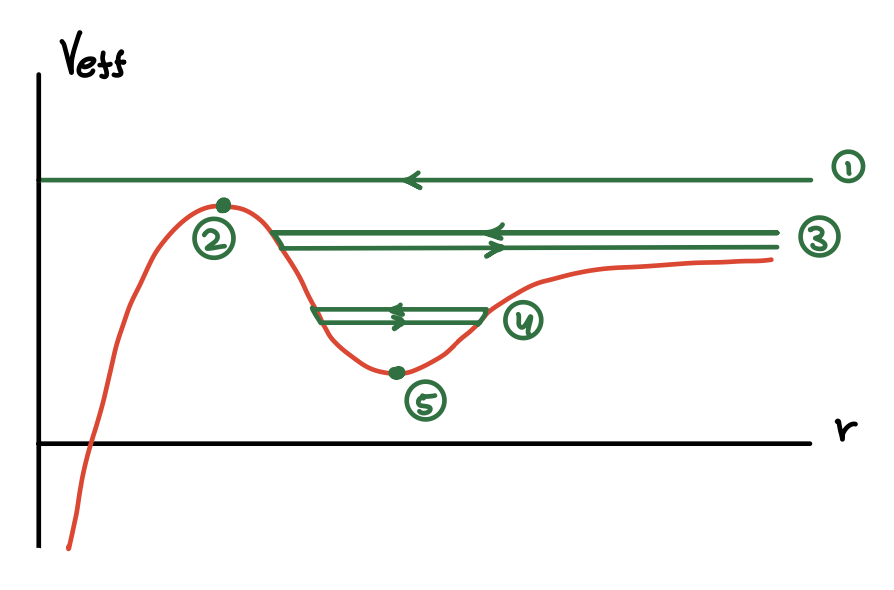
\includegraphics[scale=0.5]{veff.png}
    \quad\quad\quad
    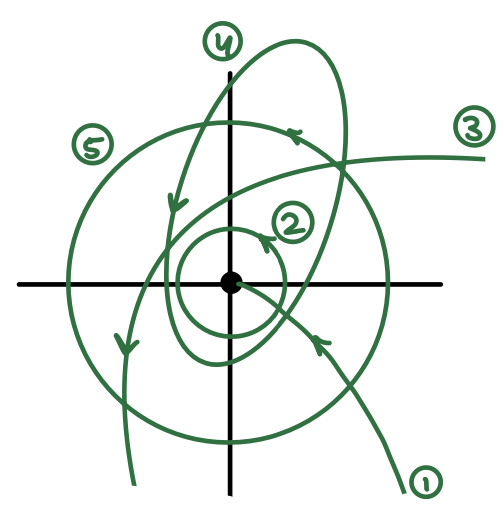
\includegraphics[scale=0.5]{orbits.png}
  \end{center}
\end{solution}

\begin{problem}{4}
Using the formula of the deflection angle in the Schwarzschild metric, $\Delta \phi_{\text{deflection}} = 4GM/c^2 b$, estimate the deflection angle of a light ray passing through the edge of Jupiter.
\end{problem}

\begin{solution}
  Plugging the appropriate constants into the formula, we get
  \[
    \Delta \phi_{\textrm{deflection}} \approx \frac{4GM}{c^2 b} = \frac{4\textrm{ rad}\times (\Gsi{6.6743e-11})\times (\kgsi{1.898e27})}{(\mpssi{3.00e8})^2\times (\msi{6.9911e7})} \times \frac{206265"}{1\textrm{ rad}} = 0.0166".
  \]
\end{solution}

\end{document}
